\begin{figure}[h]
	\centerline{
  \setlength{\tabcolsep}{2.0pt}
  \begin{tabular}{cc cc}
    %\toprule
    %\textbf{GTA5}  & \textbf{GTA5 $\rightarrow$ Cityscapes} & \textbf{Cityscapes} & \textbf{Cityscapes $\rightarrow$ GTA5}\\
	%\midrule
    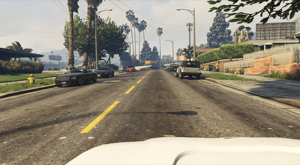
\includegraphics[width=\myw, height=\myh]{figs/gta-cityscapes/gta-00086-fs8.png} &
    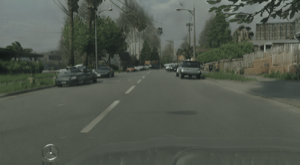
\includegraphics[width=\myw, height=\myh]{figs/gta-cityscapes/fake-cityscapes-00086-fs8.png} &
    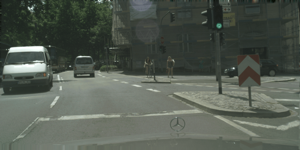
\includegraphics[width=\myw, height=\myh]{figs/gta-cityscapes/cityscapes-00086-fs8.png} &
    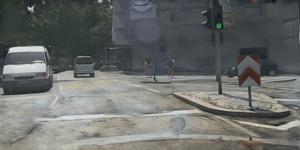
\includegraphics[width=\myw, height=\myh]{figs/gta-cityscapes/fake-gta-00086-fs8.png}
    \\
    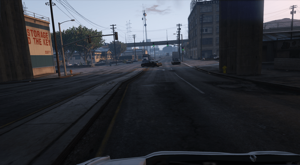
\includegraphics[width=\myw, height=\myh]{figs/gta-cityscapes/gta-00220-fs8.png} &
    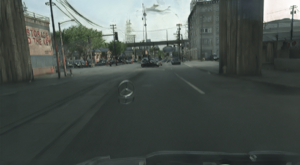
\includegraphics[width=\myw, height=\myh]{figs/gta-cityscapes/fake-cityscapes-00220-fs8.png} &
    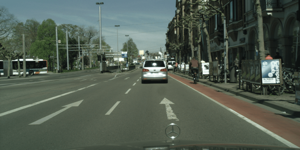
\includegraphics[width=\myw, height=\myh]{figs/gta-cityscapes/cityscapes-00220-fs8.png} &
    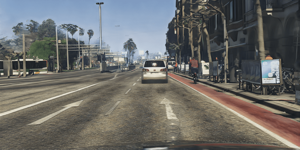
\includegraphics[width=\myw, height=\myh]{figs/gta-cityscapes/fake-gta-00220-fs8.png}
   \\
   (a) GTA5 & (b) GTA5 $\rightarrow$ Cityscapes & (c) CityScapes & (d) CityScapes $\rightarrow$ GTA5
   %\bottomrule
  \end{tabular}
  }
  \caption{%\small
  \textbf{GTA5 to CityScapes Image Translation.} Example images from the GTA5 (a) and Cityscapes (c) datasets, alongside their image-space conversions to the opposite domain, (b) and (d), respectively. Our model achieves highly realistic domain conversions.}
  \label{fig:gta-cityscapes}
\end{figure}



